
\newpage
\subsection{Problem 3 - Inequality Constrained Quadratic Programming}
From page 475 in Nocedal and Wright the following quadratic program is given.

\begin{equation}
\begin{aligned}
    \min_{x} q(x) = (x_1-1)^2+(x_2-2.5)^2 \\
    s.t. \quad x_1-2x_2+2> = 0,\\
    -x_1-2x_2+6>=0,\\
    -x_1+2x_2+2>=0,\\
    x_1>=0,\\
    x_2>=0.
\end{aligned}
\end{equation}


\textbf{Make a contour plot of the problem.}

Contour plot of the problem can be seen on figure \ref{fig:3_1}. As apparent from the plot, most of the search region is cut off by the constraints, feasible region can be seen in white.


\begin{figure}
    \centering
    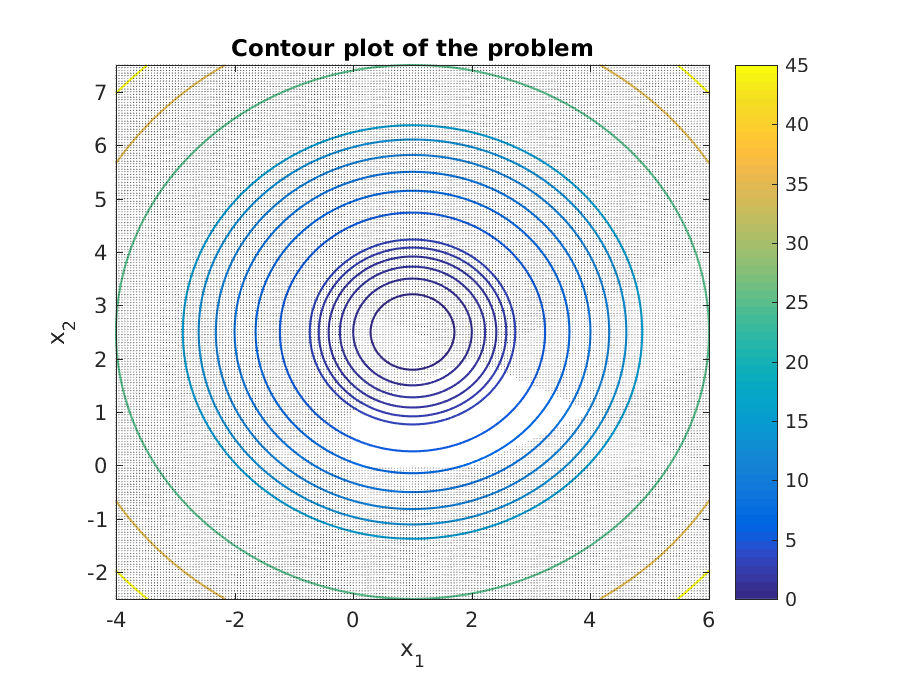
\includegraphics[width = 0.8\textwidth]{fig_3_1.eps}
    \caption{Contour plot with constraints}
    \label{fig:3_1}
\end{figure}


\textbf{Write the KKT-conditions for this problem.}

Using matrix notation the initial problem can be written as
\begin{equation}
\begin{aligned}
    \min_{x} f(x) = \frac{1}{2} x'Hx + g'x  \\
    s.t. \quad A'x \geq b, \\
\end{aligned}
\end{equation}

\[H=\begin{bmatrix}
	2 & 0 \\
	0 & 2
    \end{bmatrix}
\]

\[g=\begin{bmatrix}
	-2 \\
	-5
    \end{bmatrix}
\]

\[A=\begin{bmatrix}
    1 & -1 & -1 & 1 & 0 \\
    -2 & -2 & 2 & 0 & 1 
    \end{bmatrix}
\]

\[b= \begin{bmatrix}
    -2 \\
    -6 \\
    -2 \\
    0 \\
    0
    \end{bmatrix}
\]



Point $x^*$ is a solution if the KKT conditions are satisfied

\begin{equation}
\begin{aligned}
    Hx^* + g - A \lambda = 0  \\
    a_{i}'x^* = b_i \quad \text{for all i} \in  A(x^*) \\
    a_{i}'x^* \geq b_i \quad \text{for all i} \in I \setminus A(x^*) \\
    \lambda_i^* \geq 0 \quad \text{for all i} \in A(x^*)
\end{aligned}
\end{equation}

where $A(x^*)$ is the active set at point $x^*$.

In other words $x^*$ is a solution if gradient of the Lagrangian at that point is zero, active constraints hold with equality and inactive constraints hold i.e. $x^*$ is feasible, and lambdas are non-negative meaning it is not possible to make a step that reduces the objective while still staying feasible. 


\textbf{Argue that the KKT-conditions are both necessary and sufficient optimality conditions.}

Theorem 16.4 p.464 in N\&W and its conclusion state that if $x^*$ satisfies the KKT conditions specified above and H is positive semidefinite then $x^*$ is the unique global solution. Since H is positive definite (identity matrix multiplied by 2) and therefore also positive semidefinite, then $x^*$ is a global unique solution provided the KKT conditions are satisfied.


\textbf{Make a function for solution of convex equality constrained QPs (see Problem 1 and Problem 2).}

We used the same EqualityQPSolver function defined in problem 1. That solves the KKT system in form 

\[\begin{bmatrix}
	    H & -A \\
	    -A^T & 0
    \end{bmatrix} \times
	\begin{bmatrix}
		x\\
		\lambda
	\end{bmatrix}=
	- \begin{bmatrix}
		g\\
		b
	\end{bmatrix}
\]



\textbf{Apply a conceptual active set algorithm to the problem. Use the iteration sequence in Figure 16.3 of Nocedal and Wright. Plot the iterations sequence in your contour plot. For each iteration (guess of working set) you should list the working set, the solution, x, and the Lagrange multipliers, $\lambda$}.


The active set algorithm iteration sequence can be seen in table \ref{table:3_1} and on figure \ref{fig:3_2}. Column $x_k$ represents the position at the start of an iteration. Column $\alpha_k * p_k'$ represents the scaled step made in corresponding iteration.

\begin{center}
    \captionof{table}{Active set iterations} \label{table:3_1} 
    \begin{tabular}{c c c c c  } 
    iteration & W & $x_{k}'$ & $\alpha_k * p_k'$ & $\hat{\lambda}'$ \\ 
    \hline
    1 & 3,5 & [2, 0] & [0, 0] & [-2, -1] \\ 
    2 & 5 & [2, 0] & [-1, 0] & [-5] \\ 
    3 & $\emptyset$ & [1, 0] & [0, 1.5] & [] \\
    4 & 1 & [1, 1.5] & [0.4, 0.2] & [0.8] \\
    5 & 1 & [1.4, 1.7] & [0, 0] & [0.8] \\
    \end{tabular}
\end{center}



With the first iteration, a constraint is removed from the working set (step 0, remove negative $\lambda$ constraint), with the second iteration a step is made and a constraint is removed (step not 0, remove negative $\lambda$ constraint), with the third iteration a step is made and a blocking constraint is added to working set. With the fourth iteration a step is made and with the fifth iteration the algorithm stops (zero step, no negative $\lambda$).


\begin{figure}
    \centering
    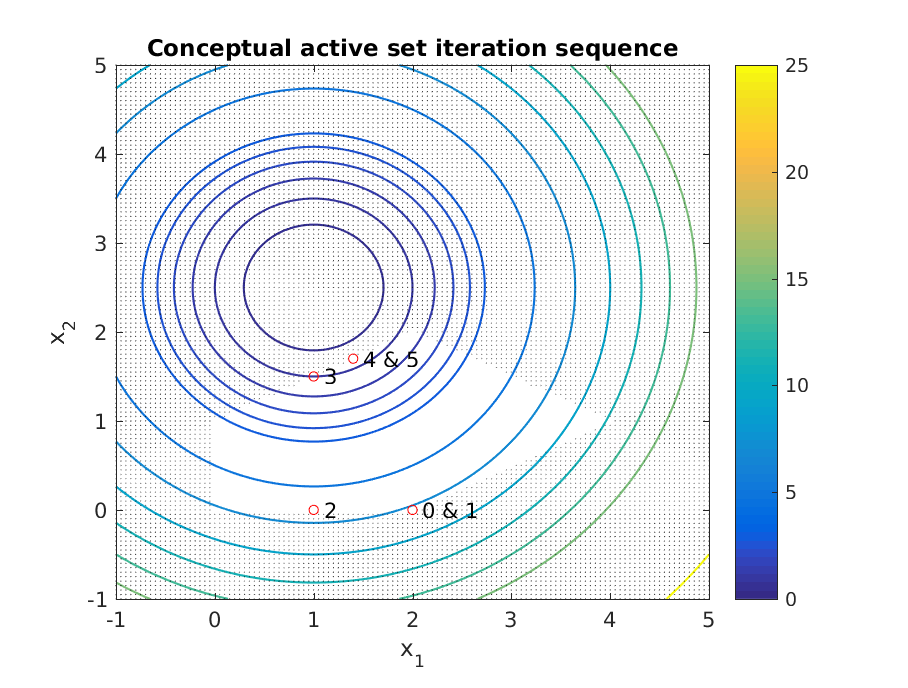
\includegraphics[width = 0.8\textwidth]{fig_3_2.eps}
    \caption{Conceptual active set iteration sequence}
    \label{fig:3_2}
\end{figure}



\textbf{Comment on the Lagrange multipliers at each iteration.}

Negative multipliers indicate that moving away from the corresponding constraint and towards the feasible region lowers the objective. The multipliers in first iteration are both negative, looking at the plot this makes sense. The starting point is at the intersection of two constraints that would not be part of the optimal active set, we could remove either for next iteration.

The Lagrange multiplier for the second iteration is -5, so moving away from this constraint likely yields a large decrease in the objective. Looking at the plot that is indeed the case, in fact, the step away from this constraint is in exactly opposite direction to the gradient of the objective function, i.e. the step is in direction of maximal rate of descent for the unconstrained problem. Since iteration 3 has empty working set, it obviously does not have any Lagrange multipliers associated with it.

With iteration 4 we move along a constraint that when looking at the plot seems to be part of the optimal working set so we expect a positive Lagrange multiplier. The multiplier is indeed positive and since at iteration 5 the step is 0 and the single $\lambda$ is still the same 0.8 (i.e. positive) the algorithm stops.


\textbf{Explain the active set method for convex QPs listed on p. 472 in N\&W.}

We start with an initial feasible point and an active set corresponding to that point. (Linear programming problem)

In each iteration we solve an equality constrained QP sub-problem using the current working set to find a step $p_k$ that would move us from the initial point for this iteration $x_k$ to the minimizer $x_k + p_k$ corresponding to the working set $W_k$. 

If $p_k$ is nonzero and making the step retains feasibility in regards to the original (inequality constrained) problem, we set $x_{k+1} = x_k + p_k$ and continue to next iteration.

If $p_k$ is nonzero but making the step does not retain feasibility, then there exists at least one constraint currently not in the working set that essentially blocks us from making the full step. In that case we make the largest possible step in direction of $p_k$ while maintaining feasibility, add one of the blocking constraints to the working set, and continue to next iteration.

If $p_k$ is zero we compute the Lagrange multipliers $\hat{\lambda}$ corresponding to the current working set. If all these multipliers are non-negative then $x^* = x_k$ is a solution to the original problem. Using $\hat{\lambda}$ and setting all multipliers corresponding to constraints not in the working set to 0 yields the multipliers for the solution $\lambda^*$. Feasibility is guaranteed since the algorithm starts with a feasible point and only allows for feasible steps.

If one of the obtained Lagrange multipliers $\hat{\lambda}$ is negative then we can move away from the corresponding constraint while reducing the objective function, this means we will remove that constraint from the working set and continue to next iteration.


\textbf{Use linprog to compute a feasible point to a QP. Apply and test this procedure to the problem in Example 16.4.}

We used linprog with empty coefficient vector f (equivalent to f(x) = 0) and the inequality constraints specified previously. Figure \ref{fig:3_3} displays the feasible starting point (0.4568, 0.0227) we obtained. 

\begin{figure}
    \centering
    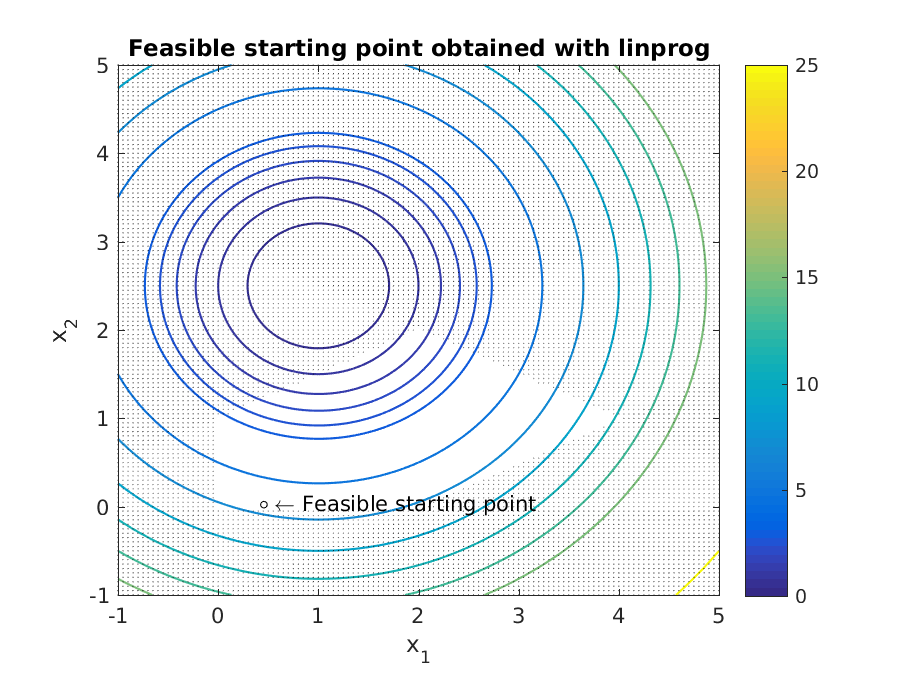
\includegraphics[width = 0.8\textwidth]{fig_3_3.eps}
    \caption{Feasible starting point}
    \label{fig:3_3}
\end{figure}

Although the point might look close to a constraint on the figure, the lambdas obtained from linprog are all effectively zero and thus the initial working set is empty.

\textbf{Implement the algorithm in p. 472 and test it it for the problem in Example 16.4. Print information for every iteration of the algorithm (i.e. the point $x_k$ , the working set $W_k$ , etc) and list that in your report.}

Running the implemented algorithm with the same initial conditions as in table \ref{table:3_1} yields the table \ref{table:3_2}. The obvious difference is that our implemented algorithm runs for 6 iterations compared to the previous conceptual algorithm that ran for 5 iterations. The difference comes from the fact that the algorithm specified in N\&W ( Algorithm 16.3) and therefore also our implementation does not remove constraints with negative Lagrange multipliers from the working set when the computed step $p_k$ was nonzero. Statements in our implementation could be restructured if smaller number of iterations is desired. Note that $alpha_k$ and $p_k'$ are separated into different columns in table \ref{table:3_2} but otherwise the tables are identical and thus our implementation correct for the particular starting conditions.



\begin{center}
    \captionof{table}{Active set test with initial point (2, 0) } \label{table:3_2} 
    \begin{tabular}{c c c c c c } 
    iteration & W & $x_{k}'$ & $p_k'$ & $\hat{\lambda}'$ & $\alpha_k$ \\ 
    \hline
    1 & 3,5 & [2, 0] & [0, 0] & [-2, -1] & -\\ 
    2 & 5 & [2, 0] & [-1, 0] & [-5] & 1\\ 
    3 & 5 & [1, 0] & [0, 0] & [-5] & -\\
    4 & $\emptyset$ & [1, 0] & [0, 2.5] & [] & 0.6\\
    5 & 1 & [1, 1.5] & [0.4, 0.2] & [0.8] & 1\\
    6 & 1 & [1.4, 1.7] & [0, 0] & [0.8] & -\\
    \end{tabular}
\end{center}



\textbf{Test your active set algorithm for the problem in Example 16.4 using (16.47) and (16.48) in N\&W. Do the same using quadprog.}

We tested our implementation as well as quadprog on inputs corresponding to the big M method with various feasible and infeasible starting points and verified that the our implementation and quadprog produce the same solutions.

